\cotefile{156-8}
\scanpage{106}
\mspage{97}
% archive sheet number: 106

\uline{Ex 3}
\[
\unsure{\Phi|\varphi}=\{S_{ab},P_b,S_{bc},P_d\},\quad
\text{\unsure{comp. connexes}}\quad \{S_{ab},P_b,S_{bc}\}\text{ et }P_d
\]
\[
\begin{aligned}
\delta\Phi&=\{a,b,c,d\}\\
\partial\Phi&=\{a,c\}\deleted{\unsure{d}}\\
\Phi^{\unsure{\bullet|\circ}}&=\{a,\unsure{c'|c},d\}
\end{aligned}
\qquad\text{\unsure{tous les trois différents}.}
\]

\uline{NB} Dans tous les cas on a.
\[
\deleted{\unsure{\Phi}}
\partial\Phi\underbrace{\subset}_{\substack{\text{\unsure{canoniq.}}\\
\text{(\unsure{n'}}\exists\ \text{plus gd \unsure{ni|ou} \inserted{plus petit} élément \unsure{dans} }L\text{ !)}}}
\Phi^\bullet\subset\delta\Phi
\]

Et \deleted{$\Phi^\bullet$ \illegible{2}} On a
\[
\partial\Phi=\left\{a\in\delta\Phi\ \left|\
\begin{gathered}
\inserted{\exists\,X\in\Phi\text{ avec }P_a<X,\text{ et de}}\\
\deleted{\text{ou bien }P_a\notin\Phi,\text{ mais existe }X\in\Phi\text{ où}}\\
\deleted{P_a<X}\\
\text{\inserted{plus,}\quad\inserted{quand } }P_a\in\Phi,\\
\deleted{\text{ou bien }P_a\in\Phi,\text{ alors }\unsure{\exists!}}\\
\text{cet }X\text{ est \uline{unique}}
\end{gathered}\right.\right\}
\]
\margin{\uline{NB} Dire \uline{que} si $P_a\in\Phi$, il existe au plus un $X\in\Phi$ tel que $P_a<X$.}
\[
\begin{aligned}
={}&\text{ens. des sommets non isolés de }\Phi,\\
&\deleted{\text{\unsure{qui sont dans} }\Phi}\ \inserted{\text{qui, de plus, quand ils appartiennent à}}\\
&\deleted{\text{\unsure{qui ne}}}\ \Phi,\text{ ne sont pas ``intérieurs'' à }\Phi
\end{aligned}
\]
\[
\Phi^\bullet\underset{\text{\unsure{canoniq.}}}{=}\partial\Phi\amalg\Phi_{\mathrm{isol}}
\qquad
\begin{gathered}
\text{où }\Phi_{\mathrm{isol}}\text{ est l'ens}\\
\text{des \unsure{ponctuels} isolés de }\Phi
\end{gathered}
\]

Dans $\unsure{\mathscr{M}|\mathcal{M}}$, on va introduire une relation d'ordre, en écrivant
\[
X\underset{\mathrm{pos}}{<}Y
\left\{
\begin{array}{lll}
\text{a)}&X=P_x,\ Y=P_y&x<y\\
\text{b)}&X=P_x,\ Y=S_{ab}&x\leq a<b\\
\text{c)}&X=S_{ab},\ Y=P_y,&a<b\leq y\\
\text{d)}&X=S_{ab},\ Y=S_{a',b'}&a<b\leq a'<b'
\end{array}\right.
\]
% margin note written slanted
\margin{\uline{NB} l'indice pos dans $\underset{\mathrm{pos}}{<}$ est inutile, si on n'a pas \unsure{bloqué} les signes $<,\leq$ pour la relation d'incidence \unsure{ici} dans $\mathscr{M}$\unsure{..}.}
\[
X\underset{\mathrm{pos}}{<}Y\ \Longleftrightarrow\ :\ X\mathrel{|\circ|}Y\text{ et }
\underbrace{\operatorname{or}(\delta X)}_{\substack{\deleted{\text{\unsure{él.}}}\inserted{\text{plus petit}}\\\text{\unsure{élément}}\\\text{de }\delta X}}
<\underbrace{\operatorname{ex}(\delta Y)}_{\substack{\text{plus gd}\\\text{él. de}\\\delta Y}}
\]

\scanpage{107}
\mspage{98}
% archive sheet number: 107

En d'autres termes, on a \unsure{trouvé} une relation d'ordre sur $\unsure{\mathscr{M}|\mathcal{M}}$, telle que la relation $X\mathrel{|\circ|}Y$ dans $\mathscr{M}$ \unsure{soit|est} la relation de disjonction \deleted{\unsure{la}} associée
\[
X\mathrel{|\circ|}Y\quad\Longleftrightarrow\quad X\underset{\mathrm{pos}}{<}Y\text{ ou }Y\underset{\mathrm{pos}}{<}X
\]

Si $\unsure{\Phi|\varphi},\Psi$ sont deux parties quelconques de $\mathscr{M}$, on posera
\[
\Phi\underset{\mathrm{pos}}{<}\Psi\quad\overset{\mathrm{def}}{\Longleftrightarrow}\quad
\begin{gathered}
\forall\,X\in\Phi,Y\in\Psi,\\
X\underset{\mathrm{pos}}{<}Y
\end{gathered}
\]
\inserted{\uline{NB} Si $\Phi,\Psi$ des \unsure{préfigures} (et \unsure{si} $\Phi\underset{\mathrm{pos}}{<}\Psi$), $\Phi\cup\Psi$ \unsure{itou}\unsure{...}}

\unsure{On redonne|On retrouve} la relation d'ordre sur $L^{\unsure{\circ|''}}$ envisagée précédemment, en interprétant les drapeaux comme des parties de
\[
L^{\unsure{''|\circ}}\simeq\mathscr{M}_0\subset\mathscr{M}.
\]
\deleted{Ceci}

% margin note written slanted
\margin{\unsure{préfigures}\par
\uline{NB} Si $\Phi\underset{\mathrm{pos}}{<}\Psi$, alors
\deleted{$\delta\Phi\underset{\mathrm{pos}}{<}\delta\Psi$ ou}
\deleted{$\delta\Phi\cap\delta\Psi=\{a\}$, $a=\operatorname{ex}(\delta\Phi)=\operatorname{or}(\delta\Psi)$}
\deleted{$\unsure{\Phi\cap\Psi=\varnothing}$ et alors $P_a\notin\Phi\cap\Psi$}
$\delta\Phi\cap\delta\Psi=\varnothing$ ou de cardinal $1$.
$\Phi\cap\Psi=\varnothing$, et si $a\in\delta\Phi\cap\delta\Psi$, on a $\deleted{\unsure{\Phi}}a=\operatorname{ex}(\delta\Phi)$ $a=\operatorname{or}(\delta\Psi)$
\par
$\Phi\underset{\mathrm{pos}}{<}\Psi\Longleftrightarrow\operatorname{ex}\Phi<\deleted{\unsure{\Phi}}\operatorname{or}\Psi$
\uuline{ou} $\operatorname{ex}\Phi=\operatorname{or}\Psi$, soit $a$ \uline{et} $P_a\notin\Phi\unsure{\cap|\cup}\Psi$.}

Dans le cas où $\Phi,\Psi$ sont des \unsure{ens.} admissibles, on va introduire une relation un peu plus forte
\[
\Phi\overset{\unsure{!|'|1}}{\underset{\deleted{\mathrm{pos}}}{\unsure{\ll|<}}}\Psi
\quad\overset{\mathrm{def}}{\Longleftrightarrow}\quad
\left\{
\begin{gathered}
\Phi\overset{\deleted{\unsure{!}}}{\underset{\mathrm{pos}}{<}}\Psi,\quad\deleted{\unsure{a}}\text{ et \deleted{\unsure{si}}\inserted{lorsque}}\\
\operatorname{ex}\Phi=\operatorname{or}\Psi\text{ (soit }a\text{), on a}\\
P_a\notin\Phi,\ P_a\notin\Psi
\end{gathered}\right.
\]

i.e. on exclut un cas comme
\figure{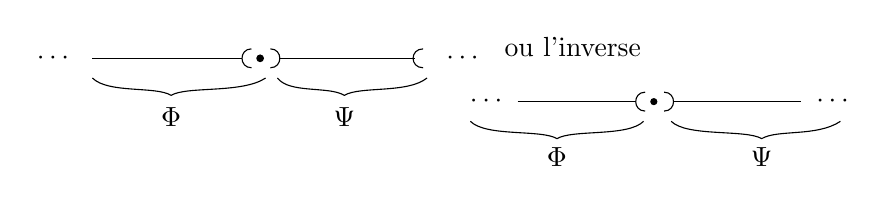
\begin{tikzpicture}[x=1cm,y=1cm]
\node at (-.5,0) {$\cdots$};
\draw (0,0)--(1.9,0);
\draw (2.02,.12) .. controls (1.86,.12) and (1.86,-.12) .. (2.02,-.12);
\fill (2.13,0) circle (1.4pt);
\draw (2.26,.12) .. controls (2.42,.12) and (2.42,-.12) .. (2.26,-.12);
\draw (2.38,0)--(4.1,0);
\draw (4.2,.12) .. controls (4.03,.12) and (4.03,-.12) .. (4.2,-.12);
\draw (0,-.25) .. controls (.2,-.45) and (.8,-.35) .. (1,-.47) .. controls (1.2,-.35) and (1.9,-.45) .. (2.2,-.25);
\draw (2.35,-.25) .. controls (2.5,-.45) and (3,-.35) .. (3.2,-.47) .. controls (3.4,-.35) and (4,-.45) .. (4.25,-.25);
\node at (1,-.75) {$\Phi$};\node at (3.2,-.75) {$\Psi$};
\node at (4.7,0) {$\cdots$};
\node at (6.1,.15) {\unsure{ou l'inverse}};
\node at (5.0,-.55) {$\cdots$};\draw (5.4,-.55)--(6.9,-.55);
\draw (7.02,-.43) .. controls (6.86,-.43) and (6.86,-.67) .. (7.02,-.67);
\fill (7.13,-.55) circle (1.3pt);
\draw (7.26,-.43) .. controls (7.42,-.43) and (7.42,-.67) .. (7.26,-.67);
\draw (7.38,-.55)--(9,-.55);\node at (9.4,-.55) {$\cdots$};
\draw (4.8,-.8) .. controls (5,-1) and (5.7,-.9) .. (5.9,-1.02) .. controls (6.1,-.9) and (6.8,-1) .. (7,-.8);
\draw (7.35,-.8) .. controls (7.55,-1) and (8.3,-.9) .. (8.5,-1.02) .. controls (8.7,-.9) and (9.2,-1) .. (9.5,-.8);
\node at (5.9,-1.25) {$\Phi$};\node at (8.5,-1.25) {$\Psi$};
\end{tikzpicture}}

\scanpage{108}
\mspage{99}
% archive sheet number: 108

Cas de ``\unsure{raccord}'', \deleted{quand $\unsure{\Phi|\varphi}$} En d'autres termes, on exclut le cas où $\Phi,\Psi$ seraient des parties \inserted{\unsure{à la fois}} ouvertes et fermées de $\Phi\cup\Psi$.

Ceci posé, voici la structure d'une préfigure quelconque, en termes des préfigures connexes.

\deleted{Si on a}
\inserted{Soit}
\[
D=\{\Phi_1\underset{\deleted{\mathrm{pos}}}{\overset{\unsure{!|'|1}}{\unsure{\ll|<}}}\Phi_2
\underset{\deleted{\mathrm{pos}}}{\overset{!}{\ll}}\cdots
\underset{\deleted{\mathrm{pos}}}{\overset{!}{\ll}}\Phi_n\}
\]
un drapeau \deleted{\unsure{pour}} de $\operatorname{Préfig}_{\mathrm{conn}}(\deleted{\unsure{\Phi}}\unsure{\mathscr{M}|\mathcal{M}})$
\[
D\in{\unsure{\operatorname{Drap}}}_{<^!}^{*}(\operatorname{Préfig}_{\mathrm{conn}}(\mathscr{M}))
\]
on lui associe la préfigure
\[
\Phi_D=\bigcup_{\Phi\in D}\Phi\ \deleted{\unsure{\amalg}}\ =\bigcup_{i\in[1,n]}\Phi_i.
\]
(réunion disjointe). On a fait ce qu'il fallait pour que les $\Phi_i$ soient les comp. connexes de $\Phi$. On \unsure{trouvera} que dans le cas général \deleted{\unsure{les}} les figures s'obtiennent comme ça, i.e.

\uline{Lemme} Soient $\Phi,\Psi$ préfigures connexes, Pour que $\Phi\cap\Psi=\varnothing$ et $\Phi\cup\Psi$ soit une préfigure, \deleted{\unsure{et on a|il suffit} $\Phi\underset{\mathrm{pos}}{<}\Psi$,} il \unsure{f et s|f. et s.} que $\Phi\underset{\mathrm{pos}}{<}\Psi$. Pour que $\Phi$ \deleted{et $\Psi$ soient}

\scanpage{109}
\mspage{100}
% archive sheet number: 109

et $\Psi$ soient les comp. connexes de $\unsure{\Phi|\varphi}\cup\Psi$, i.e. $\Phi\cup\Psi$ disconnexe, il f. et s. que $\Phi\overset{\unsure{!|'|1}}{<}\Psi$ ou $\Psi\overset{!}{<}\Phi$, i.e.
\[
\{\Phi,\Psi\}\in\operatorname{Drap}_{<^!}(\operatorname{Préfig}_{\mathrm{conn}}(\unsure{\mathscr{M}|\mathcal{M}})).
\]

En résumé, on trouve donc la petite proposition récapitulative

\uline{Théorème} 1) Pour tout $\unsure{\mathbb{D}|D}\in\operatorname{Drap}^{*}(L)$, et toute partie $\alpha$ de $\unsure{\partial|\delta}\mathbb{D}$ (cf\unsure{...}), soit $\Phi_{\mathbb{D},\alpha}=F_{\mathbb{D}}\setminus\alpha$, où $F_{\mathbb{D}}$ est la figure formée des strates \unsure{interstitielles} du drapeau $D$.
\margin{$\partial D=\left\{\begin{aligned}&\varnothing\text{ si }\operatorname{card}D=1\\&\{\operatorname{or}D,\operatorname{ex}D\}\text{ si}\\&\quad\operatorname{card}D\geq2\end{aligned}\right.$}

On trouve ainsi une bijection
\[
(\mathbb{D},\alpha)\unsure{\longmapsto|\longrightarrow}\Phi_{\mathbb{D},\alpha}
\]
de l'ens des paires $D,\alpha$ sur l'ens des préfigures connexes.

2) Pour que $\Phi$ soit une figure i.e. fermée, il f. et s. que $\alpha=\varnothing$. Pour que $\Phi$ soit ouverte, \deleted{\unsure{et on a}} il f. et s., (en admettant Hyp) \deleted{\unsure{que et}} et en supposant que $L$ n'a pas de plus petit ni de plus grand élément, que \deleted{$\alpha$} $\operatorname{card}\mathbb{D}\geq2$ et $\alpha=\partial\mathbb{D}$. En \deleted{\unsure{disposant par}} admettant Hyp. et sans \unsure{préjudice|préjuger} s'il existe un plus petit ou

\scanpage{110}
\mspage{101}
% archive sheet number: 110

plus grand élément dans $L$, soit \deleted{$\unsure{\delta}$} $\Theta$ \deleted{l'ens} \unsure{la} partie de $L$, de cardinal $\{0,1,2\}$, formée desdits éléments. Alors $\unsure{\Phi|\varphi}$ est ouverte sss
\[
\deleted{\alpha=\partial D}\quad\operatorname{card}D\geq2\text{ et }\alpha=\partial\unsure{\mathbb{D}|D}-(\partial D\cap\Theta).
\]

3) Pour \unsure{tout|toute} \deleted{\unsure{suite de préfigures connexes,}}\inserted{\deleted{\unsure{de}} drapeau}
\[
D=\{\Phi_1\overset{\unsure{!|'}}{<}\Phi_2\overset{!}{<}\cdots\overset{!}{<}\Phi_n\}
\]
dans l'ens ordonné des préfigures \unsure{0-connexes},
\[
D\in\operatorname{Drap}_{<^!}^{*}(\operatorname{Préfig}_{\mathrm{conn}}(\unsure{\mathscr{M}|\mathcal{M}})),
\]
soit
\[
\Phi_D\equiv\bigcup_{\unsure{\Psi|\Phi}\in D}\Phi=\bigcup_{1\leq i\leq n}\Phi_i.
\]
C'est une réunion disjointe, et \deleted{la} $\Phi$ est une préfigure, admettant les $\Phi\in D$ comme composantes connexes.

L'application
\[
D\longmapsto\Phi_D=\bigcup_{\Phi\in D}\Phi
\]
\[
\operatorname{Drap}_{<^!}^{*}(\operatorname{Préfig}_{\mathrm{conn}}(\mathscr{M}))\longrightarrow\operatorname{Préfig}(\mathscr{M})
\]
est bijective. \deleted{Pour}

4) Pour que $\Phi_D$ soit fermée, il f. et

\scanpage{111}
\mspage{102}
% archive sheet number: 111

suffit que les $\unsure{\Phi|\varphi}\in D$ composantes le soient. Pour que $\Phi_D$ soit ouverte, il f. et s. que les $\Phi\deleted{\unsure{\subset}}\in D$ le soient.
% margin note written slanted
\margin{\unsure{Ces deux énoncés|Ces deux derniers} \unsure{deux} faits sont des faits de topologie générale dans $\unsure{\mathscr{M}|\mathcal{M}}$, muni de $\unsure{\underline{\Delta}|\trianglelefteq}$.}

Dans cette description des préfigures et des figures, la relation $\overset{\circ}{\ll}$ n'est pas intervenue encore, ni (explicitement) la relation $\mathrel{|\circ|}$ --- à sa place, c'est la relation plus explicite $\underset{\mathrm{pos}}{<}$ (ou simplement $<$) dans $\mathscr{M}$ qui nous a servi. Mais maintenant que je passe aux supports, il n'en sera pas de même.

Il faut ensuite donner une détermination explicite du support d'une préfigure quelconque. Cela se fera en plusieurs étapes

\textcircled{\scriptsize $1^{\circ}$} Énoncé ``\unsure{additif|relatif}'' : si \unsure{la} $\Phi$ a pour composantes connexes les $\Phi_{\unsure{j|i}}$, on a
\[
\operatorname{supp}^{\circ}\Phi=\bigcup_i\operatorname{supp}^{\circ}(\Phi_i)
\]
(réunion disjointe).

$2^{\circ})$ Détermination de $\operatorname{supp}^{\circ}\Phi$ pour $\Phi$ préfigure connexe. Pour ceci, trois étapes :

\scanpage{112}
\mspage{103}
% archive sheet number: 112

\textcircled{a} Cas ``irréductibles'' des figures fermées élémentaires $\{P_a\}$, $\widetilde S_{ab}=\{S_{ab},P_a,P_b\}$, et des préfigures associées $\widetilde S_{ab}\setminus\alpha$ $(\alpha\unsure{\in|\subset}\{P_a,P_b\})$.
Le résultat ici est (voir p. 91)

\deleted{$\unsure{1^{\circ}}$}(i) Si $X\in\unsure{\mathscr{M}|\mathcal{M}}_{\unsure{\xi|q}}$, on a
% margin note written slanted
\margin{moyennant Hyp. p. 91}
\[
\operatorname{supp}X\underbrace{=}_{\substack{\text{déf de}\\\operatorname{supp}X}}\operatorname{supp}^{\circ}(\widetilde X)
\underset{\text{th.}}{=}\operatorname{Omb}(X)
\underset{\text{\unsure{tautol.}}}{=}\{Z\in\mathscr{M}\mid |Z|\subset|X|\}
\]
en particulier
\[
\operatorname{supp}\{P_a\}=\{P_a\}
\]
\[
\operatorname{supp}\widetilde S_{ab}=\left\{\unsure{\mathbb{Z}|Z}\in\mathscr{M}\ \left|\
\begin{array}{ll}
\mathbb{Z}=P_x,&a\leq x\leq b\\
\deleted{\unsure{X}}\mathbb{Z}=S_{a',b'},&a\leq a'<b'\leq b
\end{array}\right.\right\}
\]

\deleted{$\unsure{2^{\circ}}$}(ii) Si \inserted{$X=S_{ab}$ et} $\alpha\subset\{P_a,P_b\}$, i.e. $\alpha\subset\partial X$, on a
\[
\begin{aligned}
\operatorname{supp}^{\circ}(\widetilde{\deleted{\unsure{S}}X}\setminus\alpha)&=\operatorname{supp}X\setminus\alpha\\
&=\left\{\mathbb{Z}\in\mathscr{M}\ \left|\
\begin{array}{ll}
\mathbb{Z}=P_x,&a\leq x\leq b\text{ et }x\notin\alpha\\
\mathbb{Z}=S_{a',b'},&a\leq a'<b'\leq b
\end{array}\right.\right\}
\end{aligned}
\]

Une autre façon \inserted{(plus élégante)} d'exprimer $2^{\circ}$ est ainsi; \deleted{$\forall X\in\mathscr{M}$.}

a) $\forall X\in\mathscr{M}$
\[
\operatorname{supp}^{\circ}X=\operatorname{Omb}^{\circ}X=\{Z\in\mathscr{M}\mid Z\overset{\circ}{\ll}X\}
\]
en particulier
\[
\operatorname{supp}^{\circ}S_{ab}=\left\{Z\in\mathscr{M}\ \left|\
\begin{array}{ll}
Z=P_x,&a<x<b\\
Z=S_{a',b'},&a\leq a'<b'\leq b
\end{array}\right.\right\}
\]

$\beta)$ Si $\beta\subset\partial S_{ab}$, on a
% margin note written slanted
\margin{$\alpha$ et $\beta$ sont liés par $\beta={\unsure{\complement|\mathcal{C}}}_{\partial X}\alpha$, $\alpha=\complement_{\partial X}\beta$.}
\[
\begin{aligned}
\operatorname{supp}^{\circ}(S_{ab}\cup\beta)&=\operatorname{supp}^{\circ}(S_{ab})\cup\beta=\operatorname{Omb}^{\circ}(S_{ab})\cup\beta\\
&=\left\{Z\in\mathscr{M}\ \left|\
\begin{array}{ll}
Z=P_x,&a<x<b\text{ ou }x\in\beta\\
Z=S_{a',b'},&a\leq a'<b'\leq b
\end{array}\right.\right\}.
\end{aligned}
\]

\textcircled{b} Cas général : Considérons $T\in\operatorname{Drap}^{*}(L)$, $\operatorname{card}T\geq3$, \deleted{$\alpha\in$} $a=\operatorname{or}T$, $b=\operatorname{ex}(T)$, \deleted{$\alpha$} $\alpha\subset\partial T=\{a,b\}$, \inserted{$\beta$ son compl. dans $\partial T$} $\unsure{\Phi|\varphi}=F_T\setminus\alpha$. On trouve alors :

\scanpage{113}
\mspage{104}
% archive sheet number: 113

\[
\operatorname{supp}\underset{\substack{\parallel\\\Phi_{T,\alpha}}}{\unsure{\Phi|\varphi}}
=\operatorname{Omb}(\widetilde S_{ab})\setminus\alpha
=\operatorname{Omb}^{\circ}(S_{ab})\cup\beta
\]
\hfill(réunion disjointe)

On a déjà fait \textcircled{a} plus haut, il faut prouver encore \textcircled{\scriptsize $1^{\circ}$} et \textcircled{b}.

Prouvons $1^{\circ})$. Cela résulte, par réc. sur le nb de composantes connexes, du

% Tall marginal rule alongside the lemma statement, ending before the proof.
\noindent\begin{tikzpicture}[overlay]
\draw[line width=0.4pt] (-0.3,-0.45) .. controls (-0.34,-3.5) and (-0.22,-5.8) .. (-0.15,-6.3);
\end{tikzpicture}%
\uline{Lemme} Soit $X\in\unsure{\mathscr{M}|\mathcal{M}}$, et soient $\Phi,\Psi$ deux parties de $\mathscr{M}$ (préfigures ?) telles que
\[
\Phi\underset{\mathrm{pos}}{<}X<\Psi
\]
% margin note written slanted
\margin{Oui, il faut supposer $\Phi,\Psi$ des préfigures.}

[NB si $\Phi$ et $\Psi$ sont des préfigures, l'existence d'un tel $X$ équivaut à $\Phi\overset{\unsure{!|'}}{<}\Psi$ : si $\operatorname{ex}\delta\Phi\unsure{=|\leq}a<\operatorname{or}\delta\Psi=b$, on prend $X=S_{ab}$. Si $a=b$, on prend $X=P_a$].

Alors
\[
\operatorname{supp}^{\circ}(\Phi\cup\Psi)=\operatorname{supp}^{\circ}(\Phi)\cup\operatorname{supp}^{\circ}(\Psi)
\]

\uline{Démonstration} On a évidemment $\unsure{\supset|>}$, il faut prouver $\subset$, i.e.
\[
Z\in\operatorname{supp}^{\circ}(\Phi\cup\Psi)\overset{?}{\Longrightarrow}Z\in\operatorname{supp}^{\circ}\Phi\text{ ou }Z\in\operatorname{supp}^{\circ}\Psi.
\]
\deleted{\unsure{Car|On}} Notons que $\Phi\underset{\mathrm{pos}}{<}X\underset{\mathrm{pos}}{<}\Psi$ implique que
\[
X\in\operatorname{cosupp}^{\circ}(\Phi\cup\Psi),
\]
donc $Z\mathrel{|\circ|}X$, ce qui signifie aussi
\[
Z\underset{\mathrm{pos}}{<}X\text{ ou }Z\underset{\mathrm{pos}}{>}X.
\]
